% Compile with: pdflatex -interaction=nonstopmode -halt-on-error GATEWay_DARS_Full_Project_Report.tex
\documentclass[12pt,a4paper]{report}

\usepackage[T1]{fontenc}
\usepackage{lmodern}
\usepackage[margin=1in]{geometry}
\usepackage{graphicx}
\usepackage{booktabs}
\usepackage{array}
\usepackage{tabularx}
\usepackage{longtable}
\usepackage{amsmath}
\usepackage{amssymb}
\usepackage{xcolor}
\usepackage{hyperref}
\usepackage{enumitem}
\usepackage{caption}
\usepackage{subcaption}
\usepackage{fancyhdr}

\hypersetup{
  colorlinks=true,
  linkcolor=blue,
  citecolor=blue,
  urlcolor=blue
}

\definecolor{gatewayBlue}{HTML}{2563EB}
\definecolor{gatewayGreen}{HTML}{16A34A}
\definecolor{gatewayPurple}{HTML}{6D28D9}
\definecolor{gatewayGray}{HTML}{475569}

\pagestyle{fancy}
\fancyhf{}
\lhead{GATEWay DARS Project Report}
\rhead{\thepage}
\setlength{\headheight}{15pt}

\title{
  \vspace{-2cm}
  \textbf{GATEWay: Adaptive GATE DA Preparation Platform}\\
  \large Complete Project Report on Dynamic Adaptive Rating, Graph-Guided Recommendation, Remediation, and Learning Analytics
}
\author{
  Sunil Kumar\\
  B.Tech Project\\
  GATEWay Adaptive Preparation Platform
}
\date{May 2026}

\begin{document}

\maketitle
\pagenumbering{roman}

\begin{center}
\textbf{Project Keywords}\\
Adaptive assessment, GATE DA, DARS, Elo, Glicko-2, knowledge graph, remediation, rapid guessing, student analytics, teacher dashboard, Supabase, React, TypeScript.
\end{center}

\chapter*{Abstract}
GATEWay is a full-stack adaptive preparation platform for GATE Data Science and Artificial Intelligence (DA). The project combines a React and TypeScript frontend, Supabase-backed data storage, role-based student and teacher workflows, question banks, adaptive tests, review screens, analytics dashboards, and research notebooks. Its main research and engineering contribution is DARS, the Dynamic Adaptive Rating System, a rating and recommendation layer designed for intelligent assessment.

DARS extends classical Elo-style rating with educational signals that fixed rating systems ignore: dynamic uncertainty-aware update factors, continuous performance quality, response-time efficiency, streak and momentum behavior, rapid-guess penalties, graph-aware item routing, remediation paths, and student-level readiness prediction. The project includes a generated 220-student bot dataset pack with 55,000 temporal interactions, 1,683 adaptive test sessions, 77,850 question-level test rows, 2,140 graph edges, and 220 student performance snapshots. A full metrics notebook compares DARS variants against Glicko-2, fixed Elo, static starting rating, and planned deep knowledge tracing baselines.

On the held-out student benchmark, the calibrated DARS$^+$ model achieves the strongest reported results: Brier score 0.2244, log loss 0.6393, accuracy 0.6306, ROC AUC 0.6319, and calibration error 0.0062. A temporal no-future-leak validation also shows DARS$^+$ improving raw DARS on the final 30\% of each student's chronological sequence. The result is both an industry-ready adaptive learning system and a reproducible research framework for future evaluation on real student data and public tutoring datasets.

\tableofcontents
\listoffigures
\listoftables
\clearpage
\pagenumbering{arabic}

\chapter{Introduction}
\section{Project Background}
GATE DA preparation requires repeated practice over a large body of mathematical, programming, machine learning, database, artificial intelligence, and statistics concepts. A conventional practice application can store tests and scores, but it does not answer the most important pedagogical questions:

\begin{itemize}[leftmargin=*]
  \item What is the student's current skill level?
  \item Which concept should the student practice next?
  \item Is a low score caused by lack of knowledge, fatigue, rapid guessing, or topic mismatch?
  \item How can a teacher identify students needing intervention?
  \item Can the platform justify its recommendations and rating updates?
\end{itemize}

GATEWay addresses these questions by combining adaptive testing with explainable analytics. The system records rich student attempts, reconstructs review payloads, recommends graph-guided next questions, and produces teacher-facing evidence.

\section{Problem Statement}
The project aims to design and implement a GATE DA preparation platform that:

\begin{enumerate}[leftmargin=*]
  \item supports student practice, adaptive tests, retakes, and review;
  \item supports teacher course management, assignment creation, roster analytics, and student profiles;
  \item maintains dynamic student ability estimates instead of static scores;
  \item recommends questions using knowledge-graph structure and weak-topic evidence;
  \item detects rapid guesses and handles remediation after missed questions;
  \item exports research-ready datasets and notebooks for model comparison.
\end{enumerate}

\section{Objectives}
The main objectives are:

\begin{itemize}[leftmargin=*]
  \item Build a usable web application for student and teacher workflows.
  \item Implement DARS as an adaptive rating and routing engine.
  \item Generate connected CSV datasets for experimentation and paper writing.
  \item Compare DARS against Glicko-2, fixed Elo, and other baselines.
  \item Produce a reproducible notebook and LaTeX report for research and project submission.
\end{itemize}

\section{Scope}
The current implementation covers a controlled simulated dataset and project-integrated question banks. It is ready for classroom trials and technical demonstration. Public dataset experiments and neural baselines such as DKT and SAKT are planned research extensions.

\chapter{Literature and Motivation}
\section{Online Rating Systems}
Elo is a simple and interpretable rating system. Given learner rating $R$ and item rating $R_q$, the expected success probability is:

\begin{equation}
E(q)=\frac{1}{1+10^{(R_q-R)/400}}.
\end{equation}

The standard update is:

\begin{equation}
R' = R + K(S-E),
\end{equation}

where $S$ is binary correctness and $K$ is a constant update factor. Elo is useful but limited because it uses a fixed $K$ and ignores educational context.

Glicko and Glicko-2 improve on Elo by modeling rating deviation and volatility. This makes uncertain ratings move more and stable ratings move less. However, Glicko-2 still treats a student response primarily as a game outcome and does not natively include response time, streaks, remediation context, or graph structure.

\section{Knowledge Tracing}
Bayesian Knowledge Tracing, Deep Knowledge Tracing (DKT), and Self-Attentive Knowledge Tracing (SAKT) model student knowledge as a sequence. These models can be powerful predictors but are less transparent than a rating system. They often need larger datasets, careful tuning, and explainability layers.

\section{Graph-Based Learning}
Educational content naturally forms a graph. Easy questions can lead to medium questions in the same topic; prerequisite concepts can connect topics; cross-domain concepts can connect subjects. A graph-based router can recommend nearby recovery questions after a miss and more challenging questions during strong performance.

\section{Motivation for DARS}
DARS is motivated by the need for a system that is:

\begin{itemize}[leftmargin=*]
  \item interpretable enough for teachers and students;
  \item dynamic enough to track skill changes;
  \item rich enough to include time, streak, remediation, and graph context;
  \item practical enough to deploy in a web application.
\end{itemize}

\chapter{System Requirements}
\section{Functional Requirements}
\begin{longtable}{p{0.18\linewidth}p{0.72\linewidth}}
\caption{Functional requirements.}\\
\toprule
Module & Requirement \\
\midrule
\endfirsthead
\toprule
Module & Requirement \\
\midrule
\endhead
Student Auth & Students can sign up, log in, join courses, and access assigned practice.\\
Teacher Auth & Teachers can manage courses, assignments, and rosters.\\
Question Bank & The platform stores GATE DA question sets with topic, subject, difficulty, marks, and answer metadata.\\
Adaptive Practice & The app serves adaptive tests and records answer-level outcomes.\\
Review & Students can review completed tests with correctness, selected answers, and explanations.\\
DARS Rating & The system updates student rating after responses using DARS logic.\\
Recommendation & The system recommends next questions using rating, weak topics, graph neighbors, and remediation state.\\
Analytics & Teachers can inspect student performance, topic weakness, progress trends, and risk signals.\\
Dataset Export & The project can generate CSV datasets and notebooks for evaluation.\\
\bottomrule
\end{longtable}

\section{Non-Functional Requirements}
\begin{itemize}[leftmargin=*]
  \item \textbf{Usability:} workflows should be clear for both students and teachers.
  \item \textbf{Reliability:} test attempts and review payloads should persist correctly.
  \item \textbf{Explainability:} recommendations and rating changes should be auditable.
  \item \textbf{Reproducibility:} datasets and notebooks should be regenerated from scripts.
  \item \textbf{Scalability:} schemas should support larger cohorts and real classroom logs.
\end{itemize}

\chapter{Technology Stack}
\section{Frontend}
The frontend is implemented with React, TypeScript, Vite, Tailwind CSS, and shadcn-style UI components. Routing uses React Router. Charts use Recharts and custom analytics components. The UI includes student pages, teacher pages, assignment workflows, test shells, and review screens.

\section{Backend and Storage}
Supabase is used for authentication, database storage, and serverless functions. The project contains student and teacher Supabase clients, migrations, role-aware tables, and helper libraries for classroom data, test history, assignments, and analytics.

\section{Research and Data Tools}
The research workflow uses:

\begin{itemize}[leftmargin=*]
  \item Node scripts for question-bank export and dataset generation;
  \item Python notebooks for analytics, graph analysis, and model comparison;
  \item CSV files for reproducible data exchange;
  \item LaTeX for report and paper generation.
\end{itemize}

\chapter{System Architecture}
\section{High-Level Architecture}
The platform can be viewed as five connected layers:

\begin{enumerate}[leftmargin=*]
  \item \textbf{Question layer:} static and generated GATE DA question banks.
  \item \textbf{Interaction layer:} student tests, responses, review payloads, and progress events.
  \item \textbf{DARS layer:} rating update, momentum, rapid-guess detection, remediation, and prediction.
  \item \textbf{Recommendation layer:} graph-guided next-question routing.
  \item \textbf{Analytics layer:} teacher dashboards, notebooks, metrics, and reports.
\end{enumerate}

\section{Major Source Modules}
\begin{table}[h]
\centering
\caption{Representative project modules.}
\begin{tabularx}{\linewidth}{lX}
\toprule
Path & Purpose \\
\midrule
\texttt{src/lib/darsRating.ts} & DARS rating update used by the app.\\
\texttt{src/lib/nextBestQuestionEngine.ts} & Question graph and recommendation logic.\\
\texttt{src/lib/studentAnalytics.ts} & Student analytics helpers.\\
\texttt{src/lib/teacherAnalytics.ts} & Teacher dashboard aggregation.\\
\texttt{scripts/generate-dars-datasets.mjs} & Generates connected DARS CSV datasets.\\
\texttt{tools/generate\_dars\_all\_metrics\_notebook.py} & Builds the full metrics comparison notebook.\\
\texttt{DARS\_All\_Metrics\_Comparison.ipynb} & Executes model comparison and graph analysis.\\
\bottomrule
\end{tabularx}
\end{table}

\chapter{Dynamic Adaptive Rating System}
\section{Learner State}
DARS represents a learner with:

\begin{equation}
s = (R, n, \sigma^2, k, m, W, Q_{ans}, \pi_{rem}),
\end{equation}

where $R$ is rating, $n$ is answered count, $\sigma^2$ is recent rating variance, $k$ is streak, $m$ is momentum, $W$ is weak-topic set, $Q_{ans}$ is answered question set, and $\pi_{rem}$ is remediation state.

\section{Dynamic K Factor}
The update factor starts high for new learners and decays as evidence accumulates:

\begin{equation}
K(n,\sigma^2)=K_{min}+(K_{max}-K_{min})e^{-\lambda \max(0,n-n_{prov})}
\frac{\sigma^2}{\sigma^2+\sigma_0^2}.
\end{equation}

This gives provisional students faster movement and settled students more stable ratings.

\section{Performance Quality}
For correct answers, DARS uses a continuous performance quality:

\begin{equation}
P(q)=w_\tau\tau(q)+w_h(1-H(q))+w_\psi\psi(k).
\end{equation}

For incorrect answers:

\begin{equation}
P(q)=\min(\epsilon_f,0.05\tau(q)).
\end{equation}

This means that response quality is not only correct or incorrect; it also considers speed, hint usage, and streak state.

\section{Rapid-Guess Detection}
A minimum solve-time estimate is computed from question length and complexity:

\begin{equation}
t_{min}(q)=\alpha_0+\alpha_1\ell_{stem}(q)+\alpha_2\ell_{opts}(q)+\alpha_3c_{idx}(q).
\end{equation}

Responses below the threshold are flagged as rapid guesses and penalized or capped.

\section{Final Rating Update}
The DARS update is:

\begin{equation}
\Delta R = K(n,\sigma^2)\phi(k)(P(q)-E(q))-\rho(q),
\end{equation}

where $\phi(k)$ is the streak multiplier and $\rho(q)$ is rapid-guess adjustment.

\chapter{Graph-Guided Recommendation}
\section{Question Graph}
The question graph is a directed weighted graph:

\begin{equation}
G=(V,E).
\end{equation}

Each node represents a question. Edges represent same-topic progression, prerequisite relationships, or cross-domain bridges.

\section{Candidate Selection}
For non-remediation mode, candidates are chosen from a bounded neighborhood:

\begin{equation}
N(q,k)=\{q' \in V : d_G(q,q') \leq k,\ q'\notin Q_{ans}\}.
\end{equation}

For remediation, candidates are related but easier:

\begin{equation}
N_r(q_m,h)=\{q' \in V : d_G(q_m,q') \leq h,\ diff(q') < diff(q_m)\}.
\end{equation}

\section{Scoring}
The recommendation score combines heuristic match and graph structure:

\begin{equation}
score(q') = w_h h(q') + w_g g(q').
\end{equation}

The heuristic component favors target difficulty, Elo match, weak-topic coverage, and type diversity. The graph component favors central nodes and pedagogically meaningful transitions.

\chapter{Dataset Generation}
\section{Bot Students}
The DARS dataset generator creates synthetic students with names, usernames, emails, passwords, personas, and starting ratings. The current default is 220 students for course join code \texttt{FTE455}.

\section{Generated Files}
\begin{table}[h]
\centering
\caption{Generated DARS dataset pack.}
\begin{tabular}{lrr}
\toprule
Dataset & Rows & Description \\
\midrule
\texttt{bot\_students\_fte455.csv} & 220 & Bot roster \\
\texttt{student\_interactions.csv} & 55,000 & Temporal practice interactions \\
\texttt{student\_test\_sessions.csv} & 1,683 & Adaptive test sessions \\
\texttt{student\_test\_question\_responses.csv} & 77,850 & Question-level responses \\
\texttt{question\_knowledge\_graph.csv} & 2,140 & Weighted question graph edges \\
\texttt{student\_performance\_snapshots.csv} & 220 & Student aggregate snapshots \\
\bottomrule
\end{tabular}
\end{table}

\section{Personas}
Bot students are assigned behavior personas such as steady improver, fast but careless, slow analytical, volatile practicer, and remediation responder. These personas control accuracy bias, speed bias, and growth rate.

\chapter{Experimental Methodology}
\section{Preprocessing}
Users with at least 10 attempted interactions are retained for reliable estimates. Each response is transformed into a model row with:

\begin{itemize}[leftmargin=*]
  \item student id and persona;
  \item question id, topic, subject, difficulty, and question Elo;
  \item correctness, response time, score, and rapid-guess flag;
  \item DARS rating before and after;
  \item graph hop distance, recommendation source, and remediation flag;
  \item streak and momentum states.
\end{itemize}

\section{Train-Test Splits}
Two leakage-safe splits are used:

\begin{enumerate}[leftmargin=*]
  \item \textbf{Held-out student split:} train on 70\% of students, test on 30\% unseen students.
  \item \textbf{Temporal split:} for each student, train on the first 70\% of chronological responses and test on the final 30\%.
\end{enumerate}

The second split ensures that no future response is used to predict an earlier response.

\section{Baselines}
\begin{itemize}[leftmargin=*]
  \item \textbf{DARS:} raw DARS expected success probability.
  \item \textbf{DARS$^+$ calibrated:} logistic calibration layer using DARS-specific signals.
  \item \textbf{Glicko-2:} rating, rating deviation, and volatility updated per adaptive test period.
  \item \textbf{Fixed Elo:} standard Elo with $K=32$.
  \item \textbf{Static start:} no-learning baseline using only starting rating.
  \item \textbf{Planned DKT/SAKT:} sequence neural baselines for future public dataset experiments.
\end{itemize}

\section{Metrics}
The evaluation computes:

\begin{itemize}[leftmargin=*]
  \item ROC AUC;
  \item accuracy at threshold 0.5;
  \item Brier score;
  \item RMSE;
  \item log loss;
  \item expected calibration error;
  \item bootstrap confidence intervals.
\end{itemize}

\chapter{Results and Analysis}
\section{Model Comparison}
\begin{table}[h]
\centering
\caption{Held-out student benchmark on 21,332 attempted responses.}
\begin{tabular}{lrrrrr}
\toprule
Model & Brier & Log loss & Accuracy & AUC & ECE \\
\midrule
\textbf{DARS$^+$ calibrated} & \textbf{0.2244} & \textbf{0.6393} & \textbf{0.6306} & \textbf{0.6319} & \textbf{0.0062} \\
Glicko-2 & 0.2308 & 0.6546 & 0.6196 & 0.6155 & 0.0468 \\
Fixed Elo & 0.2312 & 0.6551 & 0.6186 & 0.6118 & 0.0475 \\
Static start & 0.2382 & 0.6773 & 0.6169 & 0.6085 & 0.0873 \\
Raw DARS & 0.2389 & 0.6822 & 0.6191 & 0.6105 & 0.0918 \\
\bottomrule
\end{tabular}
\end{table}

\begin{figure}[h]
\centering
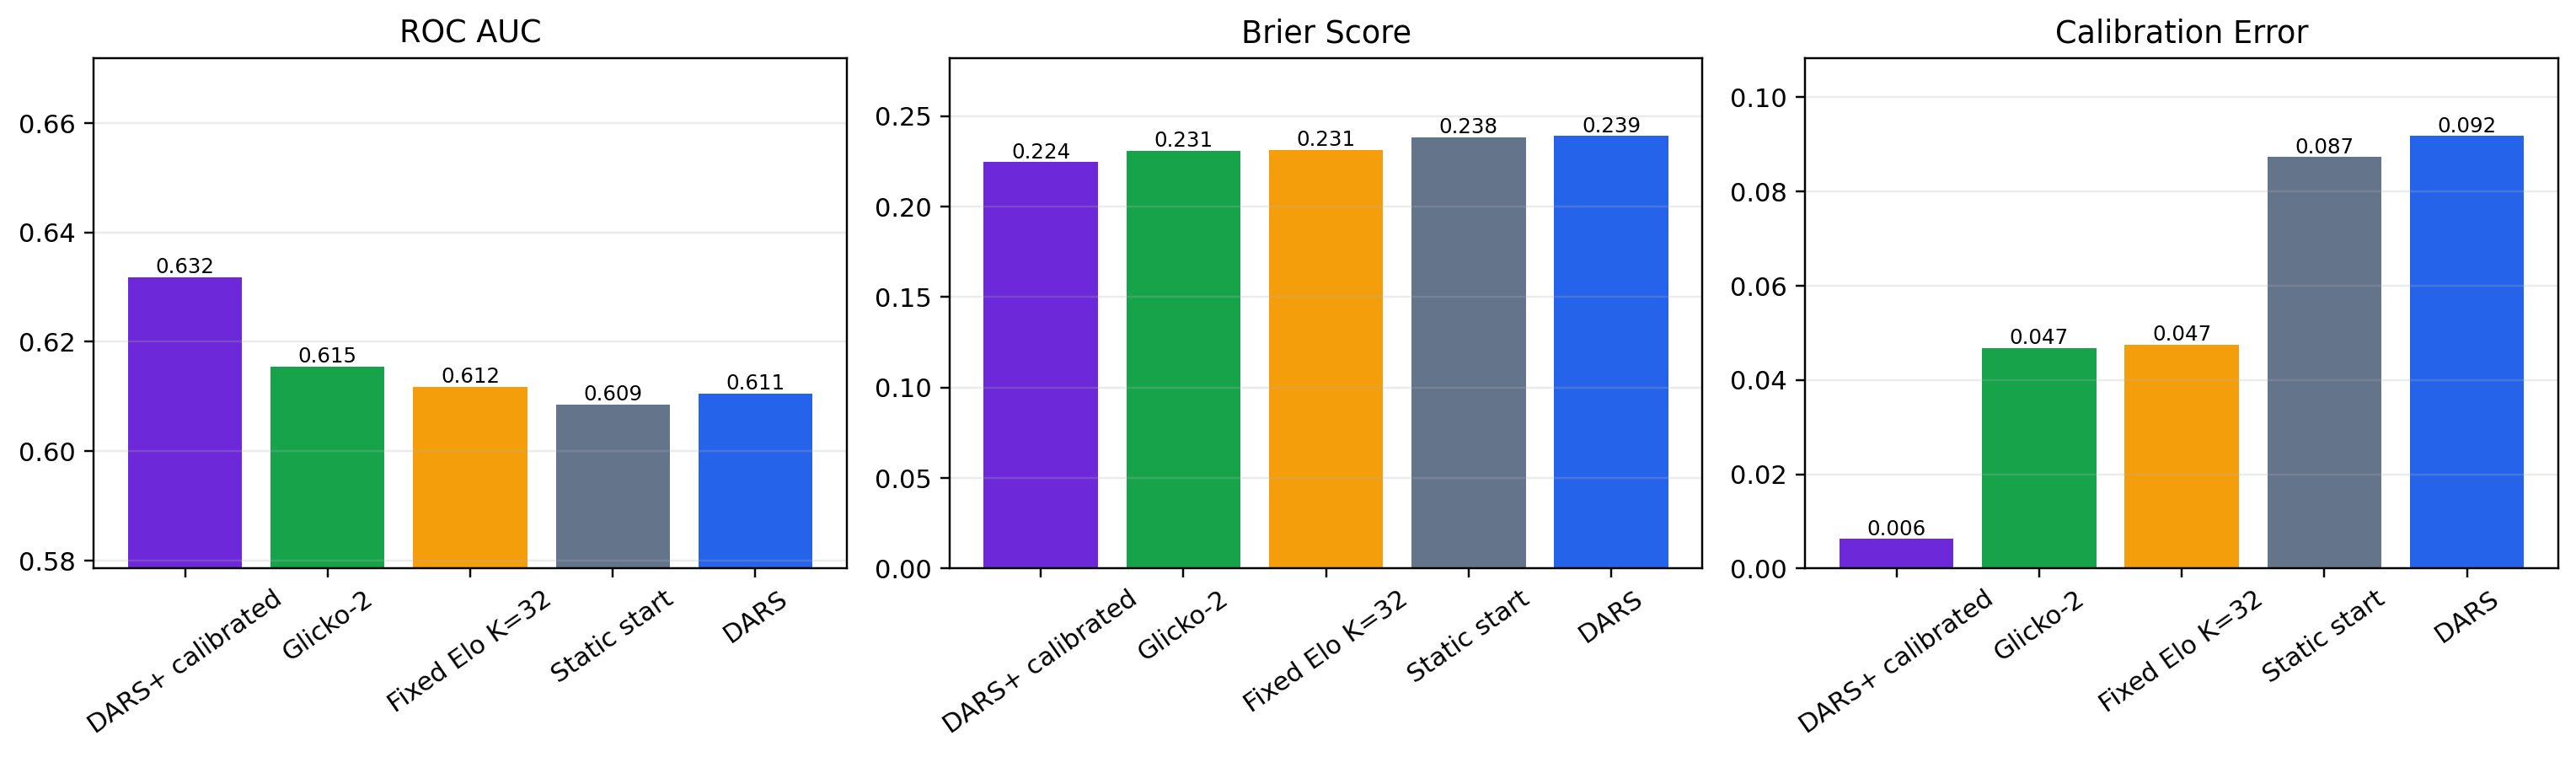
\includegraphics[width=\textwidth]{paper_figures/model_metric_comparison.png}
\caption{Model comparison across ROC AUC, Brier score, and calibration error.}
\end{figure}

DARS$^+$ performs best across all major predictive and calibration metrics. The improvement over Glicko-2 indicates that DARS-specific educational signals add predictive value beyond uncertainty-aware rating alone.

\section{Bootstrap Confidence}
\begin{figure}[h]
\centering
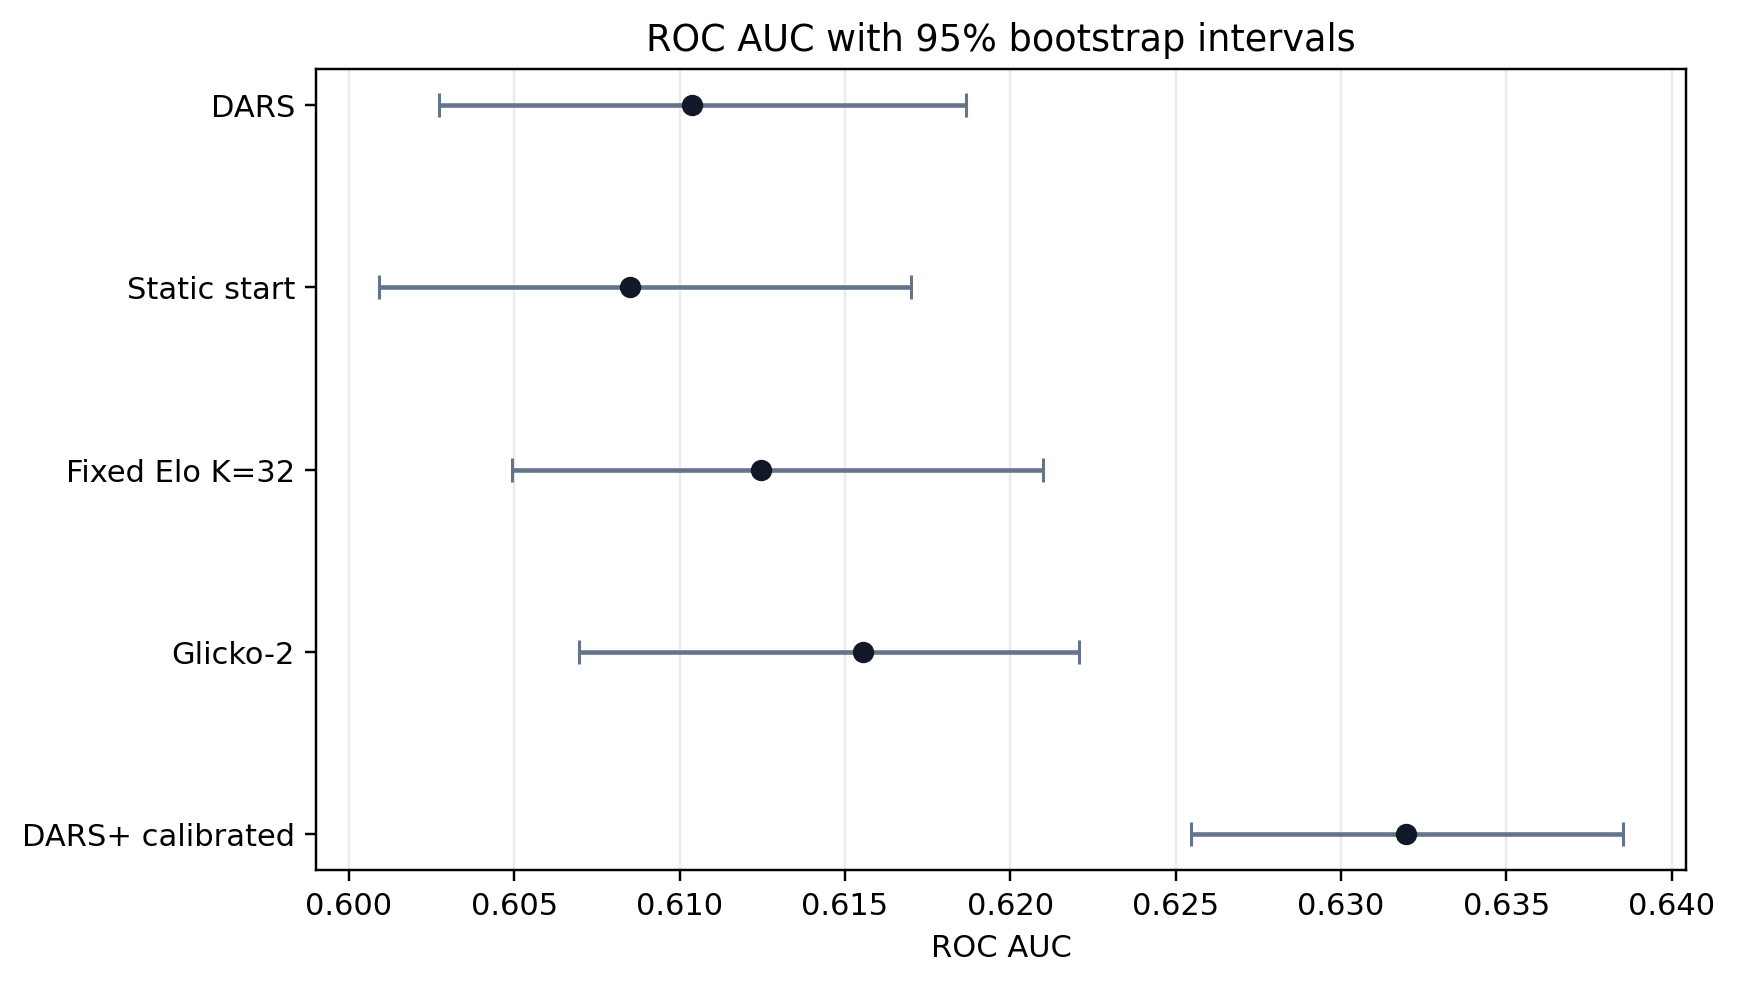
\includegraphics[width=0.85\textwidth]{paper_figures/auc_bootstrap_intervals.png}
\caption{ROC AUC bootstrap intervals for model comparison.}
\end{figure}

DARS$^+$ has ROC AUC 0.6320 with a 95\% bootstrap interval of 0.6255 to 0.6385. Glicko-2 has mean AUC 0.6156 with interval 0.6070 to 0.6221.

\section{Temporal Validation}
Under the chronological 70/30 split, DARS$^+$ reaches Brier 0.2166, log loss 0.6224, AUC 0.6422, and accuracy 0.6519. Raw DARS on the same temporal test set reaches Brier 0.2323, log loss 0.6705, AUC 0.6140, and accuracy 0.6405. This confirms that the calibrated DARS layer improves future-response prediction.

\section{Graph Routing}
\begin{figure}[h]
\centering
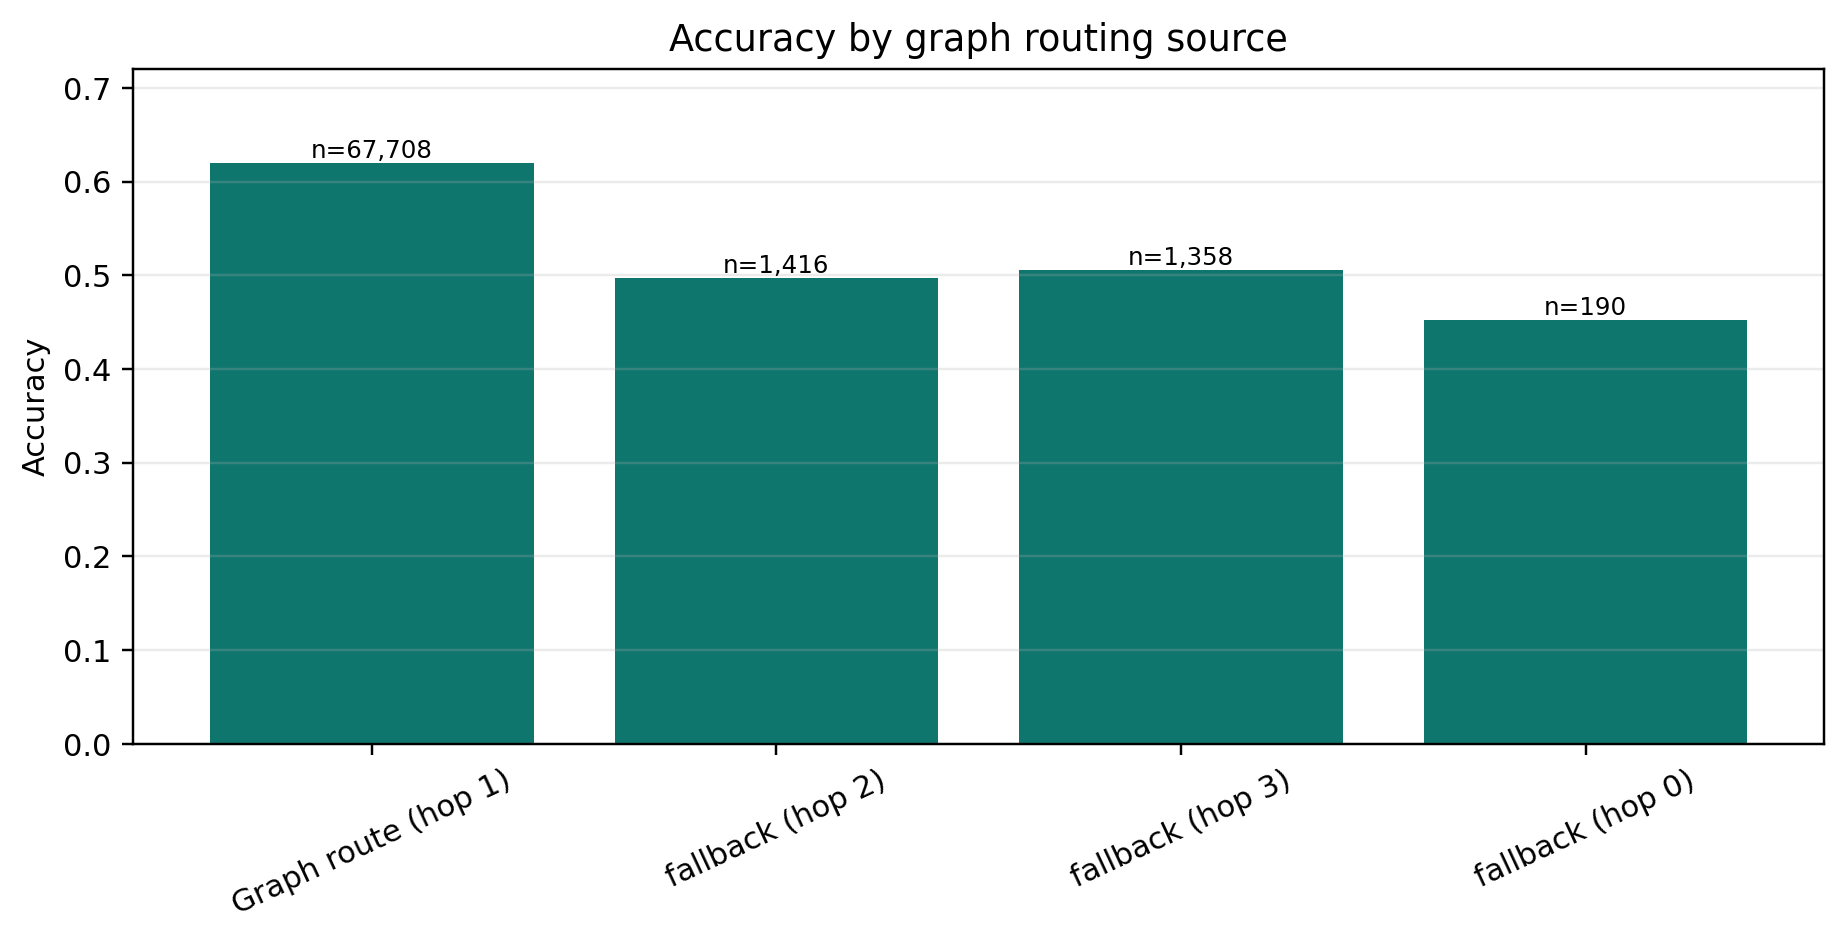
\includegraphics[width=0.85\textwidth]{paper_figures/graph_route_accuracy.png}
\caption{Accuracy by graph routing source and hop distance.}
\end{figure}

Graph-route recommendations account for 67,708 attempted responses and achieve 0.6201 accuracy. Fallback paths are less accurate, ranging from 0.4526 to 0.5059. This supports the claim that graph-neighborhood routing improves the quality of item sequencing.

\section{Remediation}
\begin{figure}[h]
\centering
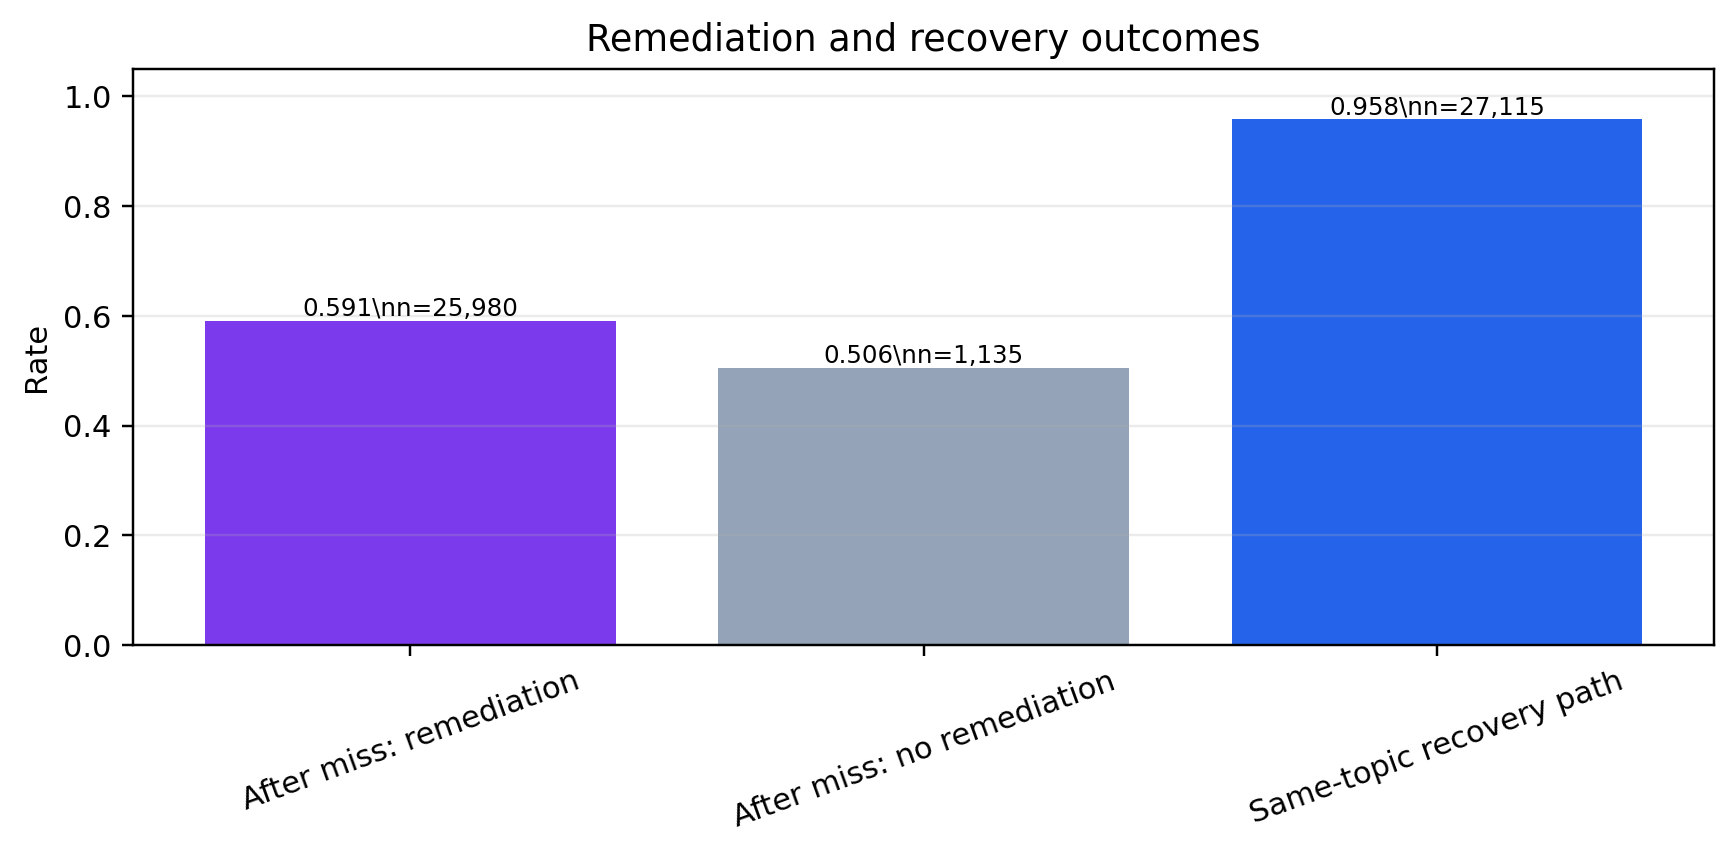
\includegraphics[width=0.85\textwidth]{paper_figures/remediation_recovery.png}
\caption{Remediation and recovery outcomes after missed questions.}
\end{figure}

After missed questions, remediation attempts achieve 0.5912 accuracy over 25,980 attempts. Non-remediation next attempts after misses achieve 0.5057 accuracy. The same-topic recovery path rate is 0.9581, showing that DARS keeps recovery work close to the failed concept.

\chapter{Implementation Details}
\section{Frontend Implementation}
The frontend is organized into reusable pages and components:

\begin{itemize}[leftmargin=*]
  \item student dashboard and course views;
  \item practice and assignment attempt pages;
  \item test history and review pages;
  \item teacher dashboard, courses, assignments, analytics, and roster pages;
  \item shared UI components and charts.
\end{itemize}

\section{Backend Integration}
Supabase provides database, authentication, and serverless function support. Separate student and teacher clients are used to support role-aware data access. Migrations define classroom, assignment, course file, activity event, and test history tables.

\section{Notebook and Report Pipeline}
The project includes reproducible notebook generation scripts. The primary metrics notebook is:

\begin{center}
\texttt{DARS\_All\_Metrics\_Comparison.ipynb}
\end{center}

It loads CSVs, computes baselines, trains DARS$^+$, evaluates held-out and temporal splits, generates graph visualizations, and exports metrics CSVs. The LaTeX report uses those CSVs and figures.

\chapter{Testing and Verification}
\section{Automated Tests}
The project includes Vitest tests for:

\begin{itemize}[leftmargin=*]
  \item DARS rating behavior;
  \item exam shell state;
  \item practice review;
  \item student analytics;
  \item gate score prediction;
  \item next-best-question engine;
  \item assignment content.
\end{itemize}

\section{Dataset Verification}
The generated manifest verifies row counts:

\begin{itemize}[leftmargin=*]
  \item 220 bot students;
  \item 55,000 interaction rows;
  \item 1,683 test sessions;
  \item 77,850 test-question rows;
  \item 220 performance snapshots.
\end{itemize}

\section{Notebook Verification}
The full metrics notebook has been executed successfully. It writes model metrics, segment metrics, student metrics, graph routing metrics, remediation metrics, and bootstrap confidence intervals.

\chapter{Industry Readiness}
\section{Operational Value}
The platform supports:

\begin{itemize}[leftmargin=*]
  \item adaptive question serving;
  \item student review and retake workflows;
  \item teacher dashboards and student profiles;
  \item bot cohorts for demonstrations and load testing;
  \item CSV exports for reporting and research.
\end{itemize}

\section{Teacher-Facing Use Cases}
Teachers can use DARS outputs to identify:

\begin{itemize}[leftmargin=*]
  \item students with low predicted readiness;
  \item high-volatility learners;
  \item weak topics and repeated misses;
  \item rapid-guess behavior;
  \item students requiring remediation.
\end{itemize}

\section{Student-Facing Use Cases}
Students can benefit from:

\begin{itemize}[leftmargin=*]
  \item adaptive practice matched to ability;
  \item transparent review of incorrect answers;
  \item recovery paths after missed questions;
  \item topic-level progress feedback;
  \item readiness estimates for GATE preparation.
\end{itemize}

\chapter{Research Roadmap}
\section{Public Dataset Evaluation}
Future work should evaluate DARS on public educational datasets such as ASSISTments and Math Garden. This requires mapping external data into student, item, concept, timestamp, correctness, and optional response-time fields.

\section{Neural Baselines}
DKT and SAKT should be implemented as sequence baselines. Hyperparameters can include hidden size, dropout, learning rate, and sequence length. Results should be reported over multiple randomized folds.

\section{Statistical Testing}
Future reports should run 10 randomized trials and report mean plus standard error. DARS should be compared to each baseline using paired tests and bootstrap confidence intervals.

\section{Graph Construction Research}
The current graph is generated from project question metadata. Future work can compare:

\begin{itemize}[leftmargin=*]
  \item expert-authored concept graphs;
  \item item-concept bipartite graphs;
  \item co-occurrence graphs;
  \item prerequisite graphs inferred from response order.
\end{itemize}

\chapter{Limitations}
\begin{itemize}[leftmargin=*]
  \item The current benchmark is based on simulated bot students, not live learners.
  \item Bot behavior may encode assumptions that favor some DARS signals.
  \item DKT, SAKT, and TrueSkill are planned but not yet fully implemented in the reported benchmark.
  \item Real-world deployment requires privacy, fairness, and monitoring checks.
  \item The graph construction method should be validated with domain experts and external datasets.
\end{itemize}

\chapter{Conclusion}
GATEWay is a complete adaptive GATE DA preparation platform with student workflows, teacher analytics, adaptive testing, review, dataset generation, and research evaluation. DARS is the central intelligence layer: it updates ratings dynamically, routes questions through a graph, detects rapid guesses, supports remediation, and produces analytics for students and teachers.

The 220-student bot dataset and metrics notebook demonstrate that DARS$^+$ outperforms Glicko-2, fixed Elo, static rating, and raw DARS on held-out student prediction and calibration. The system is therefore both a strong B.Tech software project and a credible research prototype for adaptive educational data mining.

\appendix
\chapter{Key Commands}
\begin{verbatim}
npm run export:questions
npm run generate:dars-datasets
python tools/generate_dars_all_metrics_notebook.py
jupyter nbconvert --to notebook --execute --inplace DARS_All_Metrics_Comparison.ipynb
python tools/generate_dars_report_figures.py
pdflatex -interaction=nonstopmode -halt-on-error GATEWay_DARS_Full_Project_Report.tex
\end{verbatim}

\chapter{Important Files}
\begin{longtable}{p{0.42\linewidth}p{0.48\linewidth}}
\toprule
File & Purpose \\
\midrule
\endfirsthead
\toprule
File & Purpose \\
\midrule
\endhead
\texttt{src/lib/darsRating.ts} & DARS rating implementation.\\
\texttt{src/lib/nextBestQuestionEngine.ts} & Graph recommendation engine.\\
\texttt{scripts/generate-dars-datasets.mjs} & Dataset generator.\\
\texttt{datasets/dars/manifest.json} & Dataset audit manifest.\\
\texttt{DARS\_All\_Metrics\_Comparison.ipynb} & Full model comparison notebook.\\
\texttt{DARS\_industry\_research\_paper.tex} & Short industry/research paper.\\
\texttt{GATEWay\_DARS\_Full\_Project\_Report.tex} & This full project report.\\
\bottomrule
\end{longtable}

\begin{thebibliography}{9}
\bibitem{elo}
A. E. Elo. \textit{The Rating of Chessplayers, Past and Present}. Arco, 1978.

\bibitem{glicko}
M. E. Glickman. Example of the Glicko-2 System. Technical note, 2022.

\bibitem{trueskill}
R. Herbrich, T. Minka, and T. Graepel. TrueSkill: A Bayesian Skill Rating System. In \textit{NeurIPS}, 2007.

\bibitem{dkt}
C. Piech et al. Deep Knowledge Tracing. In \textit{NeurIPS}, 2015.

\bibitem{sakt}
S. Pandey and G. Karypis. A Self-Attentive Model for Knowledge Tracing. In \textit{EDM}, 2019.

\bibitem{assistments}
N. T. Heffernan and C. L. Heffernan. The ASSISTments Ecosystem. \textit{International Journal of Artificial Intelligence in Education}, 2014.

\bibitem{darsdraft}
Anonymous Authors. DARS: A Dynamic Adaptive Rating System for Intelligent Assessment with Graph-Based Item Routing, Contextual Remediation, and Performance Prediction. Project draft, 2026.
\end{thebibliography}

\end{document}
